% SPDX-License-Identifier: CC-BY-4.0
% Figure 2 - representative CPU-mediated feedback in an ARTIQ/Sinara system.
% This is one way to react to an external event (input event -> kernel ->
% new timestamped output). Pre-scheduled RTIO outputs do not use this loop.
% Numbered markers are latency contributors, not measured values.
\documentclass[tikz, border=0pt]{standalone}
% SPDX-License-Identifier: CC-BY-4.0
% styles.tex - shared typography, colours and TikZ styles for all HeraldRT figures.
%
% Conventions used in every figure
%   optical path        red, solid, 1.2pt, open arrow head
%   electrical event    blue, solid, 0.9pt (detector pulses, herald)
%   control output      green, dashed, 0.9pt (electronics -> actuators)
%   host / config       grey, dotted
%   implemented block   solid outline     proposed block   dashed grey outline
%   asynchronous domain light amber fill  synchronous domain light blue fill

\usepackage{fontspec}
\usepackage{unicode-math}
\setmainfont{FiraSans}[
  Extension = .otf, UprightFont = *-Book, BoldFont = *-SemiBold,
  ItalicFont = *-BookItalic, BoldItalicFont = *-SemiBoldItalic]
\setsansfont{FiraSans}[
  Extension = .otf, UprightFont = *-Book, BoldFont = *-SemiBold,
  ItalicFont = *-BookItalic, BoldItalicFont = *-SemiBoldItalic]
\setmathfont{FiraMath-Regular.otf}
\setmonofont{FiraMono}[Extension = .otf, UprightFont = *-Regular, BoldFont = *-Medium,
  Scale = 0.92]
\renewcommand{\familydefault}{\sfdefault}

\usepackage[detect-all]{siunitx}
\sisetup{range-phrase = --, range-units = single, per-mode = symbol}

\usepackage{tikz}
\usetikzlibrary{arrows.meta, positioning, calc, fit, backgrounds,
  decorations.pathmorphing, decorations.markings, shapes.geometric, shapes.misc}

% layer for domain shading: above the white page, below blocks and wires
\pgfdeclarelayer{board}
\pgfdeclarelayer{domains}
\pgfsetlayers{background, board, domains, main}

% reproducible PDF (no creation date / ID differences between builds)
\pdfvariable suppressoptionalinfo 1023

% ------------------------------------------------------------------ colours
\definecolor{ink}{HTML}{1B2631}
\definecolor{optical}{HTML}{B03A2E}
\definecolor{opticallight}{HTML}{F2D7D5}
\definecolor{pumpviolet}{HTML}{6C3483}
\definecolor{elec}{HTML}{1F4E79}
\definecolor{ctrl}{HTML}{1E7B4A}
\definecolor{host}{HTML}{6E7B85}
\definecolor{asyncfill}{HTML}{FDF2E3}
\definecolor{asyncline}{HTML}{C07A1E}
\definecolor{syncfill}{HTML}{EAF2FA}
\definecolor{syncline}{HTML}{4F7FAF}
\definecolor{boxfill}{HTML}{FFFFFF}
\definecolor{muted}{HTML}{8A949C}
\definecolor{lat}{HTML}{C0392B}

\colorlet{proposed}{muted}

% ------------------------------------------------------------------ styles
\tikzset{
  every picture/.style = {line join = round, line cap = round, font = \small,
    text = ink, >={Stealth[length=2.2mm, width=1.6mm]}},
  % white page so the SVG stays readable in GitHub's dark mode
  white page/.style = {show background rectangle,
    background rectangle/.style = {fill = white, draw = none},
    inner frame xsep = 4mm, inner frame ysep = 3.5mm},
  % blocks
  block/.style = {draw = ink, line width = 0.7pt, fill = boxfill, rounded corners = 1.5pt,
    align = center, inner sep = 4pt, minimum height = 9mm},
  smallblock/.style = {block, font = \footnotesize, minimum height = 7mm, inner sep = 3pt},
  proposedblock/.style = {block, draw = proposed, dash pattern = on 3pt off 2pt,
    text = proposed, fill = white},
  device/.style = {block, fill = black!3},
  domain async/.style = {draw = asyncline, fill = asyncfill, line width = 0.6pt,
    rounded corners = 3pt, inner sep = 3.5mm},
  domain sync/.style = {draw = syncline, fill = syncfill, line width = 0.6pt,
    rounded corners = 3pt, inner sep = 3.5mm},
  board/.style = {draw = ink!70, line width = 0.7pt, rounded corners = 4pt, inner sep = 4mm},
  domain label/.style = {font = \footnotesize\bfseries, align = left},
  note/.style = {font = \footnotesize, text = ink!80, align = center},
  tag/.style = {font = \scriptsize, text = ink!70},
  % signals
  optical/.style = {draw = optical, line width = 1.2pt, -{Stealth[length=2.6mm, width=2mm]}},
  optical nohead/.style = {draw = optical, line width = 1.2pt},
  pump light/.style = {draw = pumpviolet, line width = 1.2pt, -{Stealth[length=2.6mm, width=2mm]}},
  elec/.style = {draw = elec, line width = 0.9pt, ->},
  ctrl/.style = {draw = ctrl, line width = 0.9pt, dash pattern = on 3.5pt off 2pt, ->},
  hostlink/.style = {draw = host, line width = 0.8pt, dash pattern = on 1pt off 1.6pt, <->},
  latency/.style = {circle, fill = lat, text = white, font = \scriptsize\bfseries,
    inner sep = 0.6pt, minimum size = 3.9mm},
}

% value-class tags used in the timing figure
\newcommand{\clsP}{\textsuperscript{\textcolor{optical}{\bfseries P}}}
\newcommand{\clsD}{\textsuperscript{\textcolor{asyncline}{\bfseries D}}}
\newcommand{\clsC}{\textsuperscript{\textcolor{ctrl}{\bfseries C}}}
\newcommand{\clsA}{\textsuperscript{\textcolor{host}{\bfseries A}}}


\begin{document}
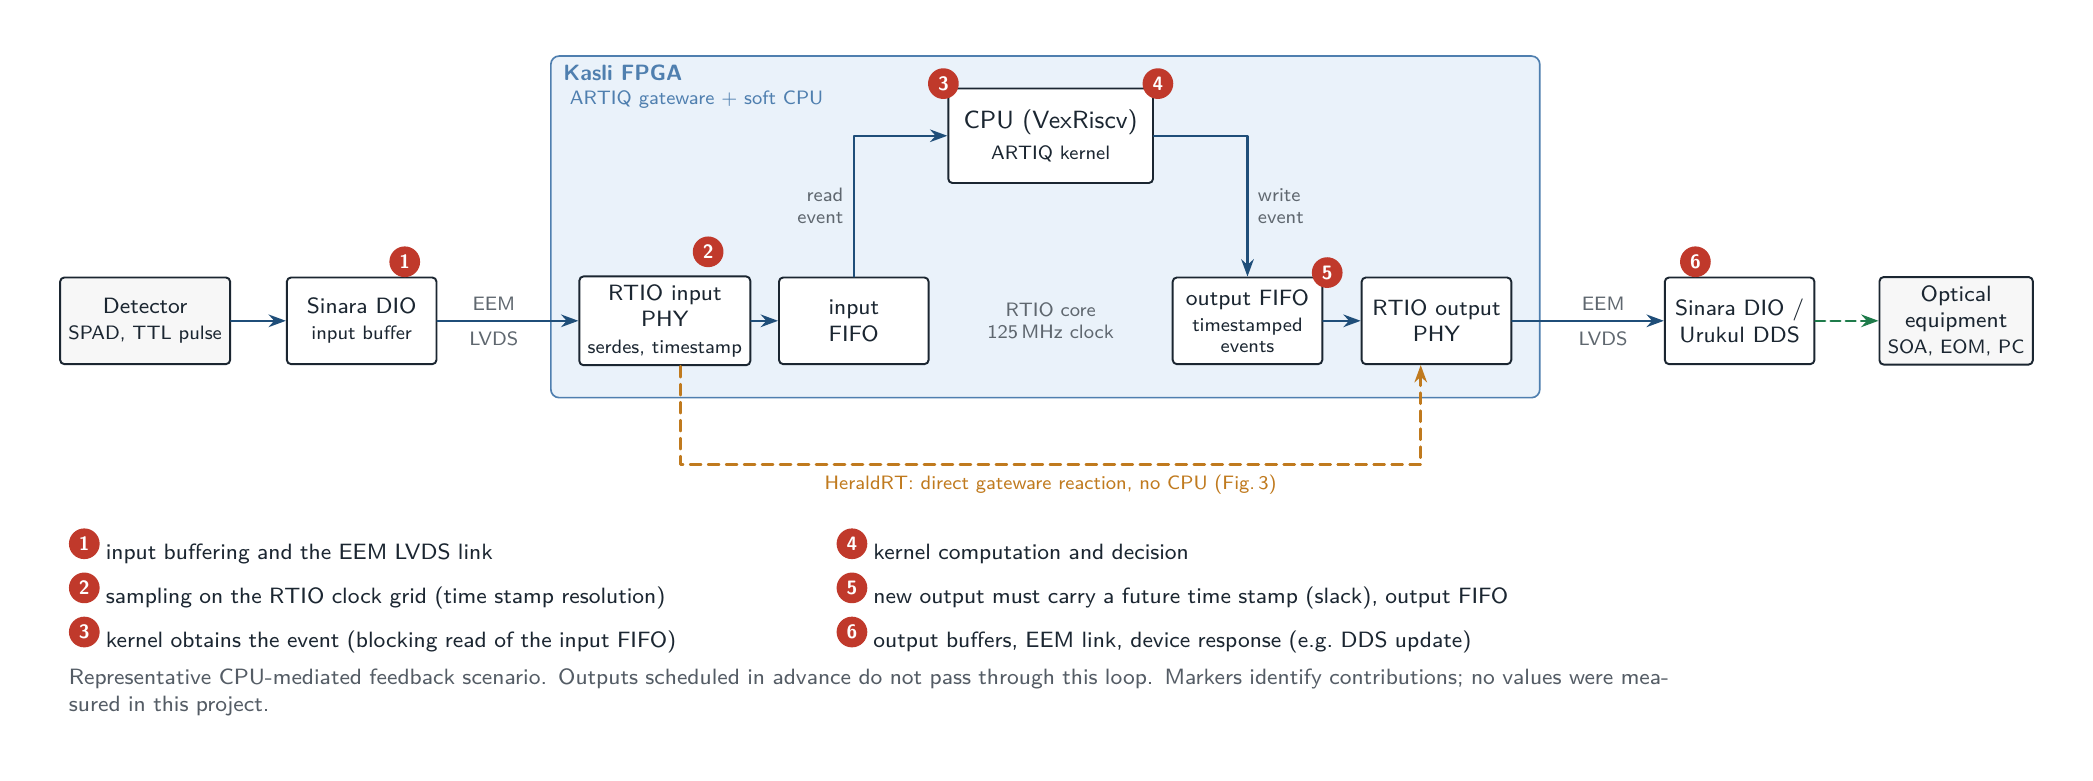
\begin{tikzpicture}[white page]
  \tikzset{stage/.style = {smallblock, minimum width = 19mm, minimum height = 11mm}}

  % ------------------------------------------------------------------ nodes
  \node[stage, fill = black!3] (det)    at (-0.9, 0) {Detector\\{\scriptsize SPAD, TTL pulse}};
  \node[stage]                 (dioin)  at (1.85, 0) {Sinara DIO\\{\scriptsize input buffer}};
  \node[stage]                 (inphy)  at (5.7, 0) {RTIO input\\PHY\\{\scriptsize serdes, timestamp}};
  \node[stage]                 (infifo) at (8.1, 0) {input\\FIFO};
  \node[block, minimum width = 26mm, minimum height = 12mm] (cpu) at (10.6, 2.35)
        {CPU (VexRiscv)\\{\scriptsize ARTIQ kernel}};
  \node[stage]                 (outfifo) at (13.1, 0) {output FIFO\\{\scriptsize timestamped}\\[-2pt]{\scriptsize events}};
  \node[stage]                 (outphy) at (15.5, 0) {RTIO output\\PHY};
  \node[stage]                 (dioout) at (19.35, 0) {Sinara DIO /\\Urukul DDS};
  \node[stage, fill = black!3] (equip)  at (22.1, 0) {Optical\\equipment\\{\scriptsize SOA, EOM, PC}};

  % Kasli region
  \begin{pgfonlayer}{domains}
    \node[domain sync, fit = (inphy) (infifo) (cpu) (outfifo) (outphy), inner ysep = 4mm,
          inner xsep = 3.5mm] (kasli) {};
  \end{pgfonlayer}
  \node[domain label, anchor = north west, text = syncline] at (kasli.north west)
       {\,Kasli FPGA\\[-1pt]{\scriptsize\mdseries\, ARTIQ gateware + soft CPU}};
  \node[tag, align = center] at ($(infifo)!0.5!(outfifo)$) {RTIO core\\\SI{125}{MHz} clock};

  % ------------------------------------------------------------------ links
  \draw[elec] (det) -- (dioin);
  \draw[elec] (dioin) -- node[above, tag, pos = 0.4] {EEM} node[below, tag, pos = 0.4] {LVDS} (inphy);
  \draw[elec] (inphy) -- (infifo);
  \draw[elec] (infifo.north) |- node[pos = 0.25, left, tag, align = right] {read\\event} (cpu.west);
  \draw[elec] (cpu.east) -| node[pos = 0.75, right, tag, align = left] {write\\event} (outfifo.north);
  \draw[elec] (outfifo) -- (outphy);
  \draw[elec] (outphy) -- node[above, tag, pos = 0.6] {EEM} node[below, tag, pos = 0.6] {LVDS} (dioout);
  \draw[ctrl] (dioout) -- (equip);

  % latency markers
  \node[latency] at ($(det.east)!0.5!(inphy.west) + (0, 0.75)$) {1};
  \node[latency] at ($(inphy.north) + (0.55, 0.3)$) {2};
  \node[latency] at ($(cpu.north west) + (-0.05, 0.05)$) {3};
  \node[latency] at ($(cpu.north east) + (0.05, 0.05)$) {4};
  \node[latency] at ($(outfifo.north east) + (0.05, 0.05)$) {5};
  \node[latency] at ($(outphy.east)!0.5!(equip.west) + (0, 0.75)$) {6};

  % the alternative (HeraldRT) - drawn for orientation only
  \draw[draw = asyncline, line width = 0.9pt, dash pattern = on 4pt off 2.5pt, ->]
       ($(inphy.south) + (0.2, 0)$) -- ++(0, -1.25) -| node[pos = 0.25, below, tag, text = asyncline]
       {HeraldRT: direct gateware reaction, no CPU (Fig.\,3)} ($(outphy.south) + (-0.2, 0)$);

  % ------------------------------------------------------------------ key
  \node[anchor = north west, text width = 205mm, font = \footnotesize, align = left]
       at ($(det.south west) + (0, -1.95)$) {%
    \begin{tabular}{@{}l@{\;}p{90mm}@{\quad}l@{\;}p{90mm}@{}}
      \tikz\node[latency]{1}; & input buffering and the EEM LVDS link &
      \tikz\node[latency]{4}; & kernel computation and decision \\[2pt]
      \tikz\node[latency]{2}; & sampling on the RTIO clock grid (time stamp resolution) &
      \tikz\node[latency]{5}; & new output must carry a future time stamp (slack), output FIFO \\[2pt]
      \tikz\node[latency]{3}; & kernel obtains the event (blocking read of the input FIFO) &
      \tikz\node[latency]{6}; & output buffers, EEM link, device response (e.g.\ DDS update) \\
    \end{tabular}\\[4pt]
    {\color{ink!75}Representative CPU-mediated feedback scenario. Outputs scheduled in advance do not
    pass through this loop. Markers identify contributions; no values were measured in this project.}};
\end{tikzpicture}
\end{document}
